\documentclass[conference]{IEEEtran}
\IEEEoverridecommandlockouts
% The preceding line is only needed to identify funding in the first footnote. If that is unneeded, please comment it out.
\usepackage{cite}
\usepackage{amsmath,amssymb,amsfonts}
\usepackage{algorithmic}
\usepackage{graphicx}
\usepackage{textcomp}
\usepackage{xcolor}
\def\BibTeX{{\rm B\kern-.05em{\sc i\kern-.025em b}\kern-.08em
		T\kern-.1667em\lower.7ex\hbox{E}\kern-.125emX}}

\usepackage{textgreek}
\usepackage{placeins}

% Subfigures
\usepackage[skip=0pt]{caption}
\usepackage[skip=0pt]{subcaption}

% PGF Plots
\usepackage{pgfplots}
\pgfplotsset{compat=newest}

\pgfplotsset{
	every axis/.append style={
		font=\footnotesize,
		ymajorgrids=true,
		xmajorgrids=true,
		grid style=dashed,
		width  = 6.0cm,
		height = 5.0cm,
	},
	every axis plot/.append style={
		mark size=1,
		mark options=solid,
		line width = 1.2pt
	},
	legend image code/.code={
		\draw[mark repeat=2,mark phase=2]
		plot coordinates {
			(0cm,0cm)
			(0.15cm,0cm)        %% default is (0.3cm,0cm)
			(0.3cm,0cm)         %% default is (0.6cm,0cm)
		};%
	}
}

% User commands
\newcommand{\mytsup}[1]{\textsuperscript{#1}}
\newcommand{\mytsub}[1]{\textsubscript{#1}}
\newcommand{\mymr}[1]{\multirow{2}{*}{#1}}
\newcommand{\mymc}[1]{\multicolumn{2}{c|}{#1}}

% Tikz externalize
\usepackage{tikz}
\usetikzlibrary{external}
\tikzexternalize[prefix=tikz/,only named=true]
\tikzexternalize

\sloppy
\begin{document}
	
	\title{Hybrid Inverter-Based Fully-Differential Amplifiers\\
		%{\footnotesize \textsuperscript{*}Note: Sub-titles are not captured in Xplore and
		%should not be used}
		%\thanks{Identify applicable funding agency here. If none, delete this.}
	}

	\author{\IEEEauthorblockN{Luis Henrique Rodovalho}
	\IEEEauthorblockA{\textit{luishenriquerodovalho@gmail.com}}
	}
	
	\maketitle
	
	\begin{abstract}
		Inverter-based OTAs (Operational Transconductance Amplifiers) are versatile and scalable analog circuit blocks, which several applications use, ranging from signal processing to analog-to-digital converters. This work presents a comparison of the basic fully-differential OTA topologies, their common-mode rejection techniques, and how the designer can mix them together to create hybrid amplifier topologies.
	\end{abstract}
	
	\begin{IEEEkeywords}
		Inverter-based amplifiers, operational transconductance amplifiers, open source PDK.
	\end{IEEEkeywords}
	
	\section{Introduction}

The humble CMOS inverter is the basis of the most common CMOS digital logic gates. However, it is much more versatile, as it can be used for many analog applications, ranging from high-speed signal processing \cite{nauta1992cmos,barthelemy2008ota} with typical supply voltages, to ultra-low voltage analog-digital converters \cite{vieru2012ultra,lv2019inverter,benvenuti2021design}. The performance of those designs relies on the system topology, but it is also dependent on the underlying OTA topologies. If their basic analog blocks can be improved in any aspect, the whole system can benefit from it. However, not everything can be improved simultaneously, as there are always trade-offs in the design.

This work presents existing basic inverter-based fully differential amplifier topologies \cite{nauta1992cmos,barthelemy2008ota,vieru2011inverter,manfredini2020ultra}, in Section \ref{sc:basic}, then presents their single-stage and two-stage hybrid amplifier topologies, in Section \ref{sc:hybrid}. Their strengths and weakness are compared by analyzing their simulation results, in Section \ref{sc:results}. Finally, Section \ref{section:conclusion}, concludes this work.

\FloatBarrier

\section{Basic Inverter-Based Amplifier Topologies}\label{sc:basic}

\begin{figure}[htbp]
	%
	\centering
	\begin{subfigure}[b]{0.49\columnwidth}
		\centerline{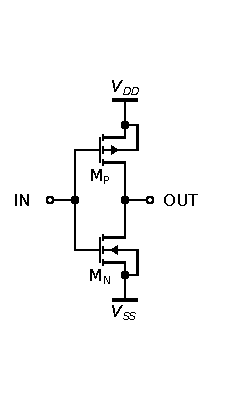
\includegraphics[scale=0.50]{circuits/inv_sch.pdf}}
		\caption{}
		\label{fig:inv:schematic}
	\end{subfigure}
	%
	\begin{subfigure}[b]{0.49\columnwidth}
		\centerline{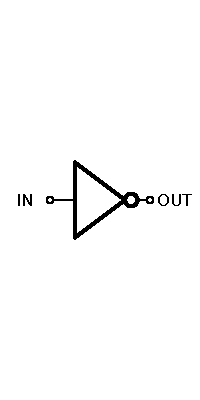
\includegraphics[scale=0.50]{circuits/inv_symbol.pdf}}
		\caption{}
		\label{fig:inv:symbol}
	\end{subfigure}\\
	%
	\begin{subfigure}[b]{0.49\columnwidth}
		\centerline{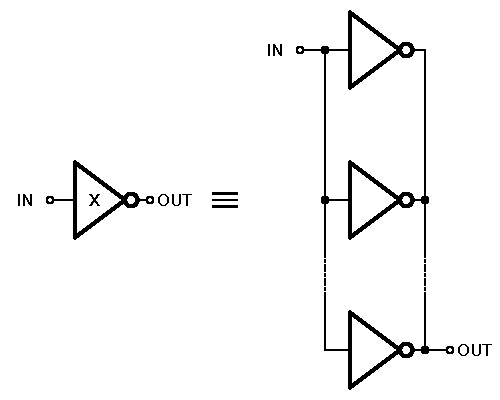
\includegraphics[scale=0.50]{circuits/inv_parallel.pdf}}
		\caption{}
		\label{fig:inv:parallel}
	\end{subfigure}
	
	\caption{(a) Single inverter symbol, (b) schematic, and (c) parallel inverters}
	\label{fig:inv:sch}
	%
\end{figure}

Figures \ref{fig:inv:schematic} and  \ref{fig:inv:symbol} shows the CMOS inverter circuit diagram and its respective symbol. Its properties, such as large and small-signal parameters, process variability, temperature and supply-voltage dependence, are thoroughly explained in \cite{rodovalho2021push}. A super inverter cell, shown in Fig. \ref{fig:inv:parallel} is made of multiple cells in parallel with shared power supplies, input and output terminals. This way, the OTA performance characteristics, such as transconductance, gain-bandwidth, power consumption, common-mode rejection ratio (CMRR), and power supply rejection ratio (PSRR), can be altered while reusing the same cell layout design.

Figure \ref{fig:nauta:sch} shows the first inverter-based amplifier topology \cite{nauta1992cmos}. It is made of six inverters, has only four nodes, and is completely symmetrical.


\begin{figure}[!htbp]
	\centerline{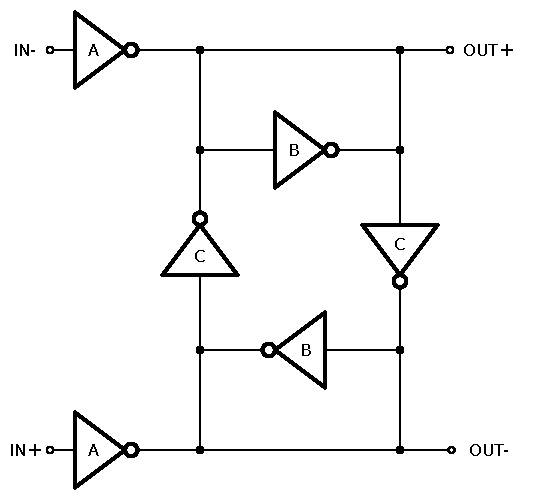
\includegraphics[scale=0.50]{circuits/nauta.pdf}}
	\caption{(N)auta OTA circuit diagram \cite{nauta1992cmos}}
	\label{fig:nauta:sch}
	%
\end{figure}

 Figure \ref{fig:barth:sch} shows another inverter-based OTA based on the common-mode input feedforward common-mode rejection technique \cite{barthelemy2008ota}, and has an extra node, for a common-mode path. The amplifier shown in Figure \ref{fig:vieru:sch} is composed of the same number of cells, but the common-mode signal path direction is reverted, so the common-mode signal is fed back to the input. This topology is useless alone, as it depends on the OTA input load, but can be useful as a cascaded second stage \cite{vieru2011inverter}.

\begin{figure}[htbp]
	%
	\centering
	\begin{subfigure}[b]{0.45\columnwidth}
		\centerline{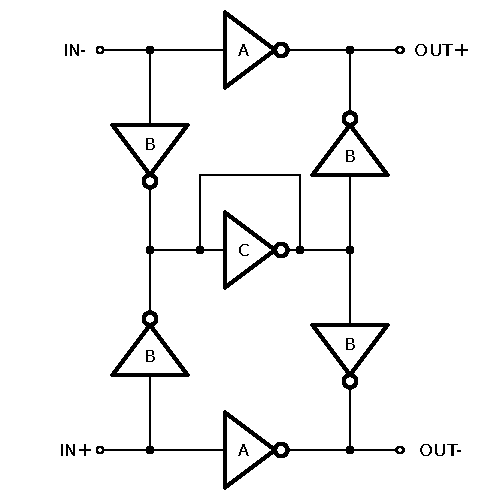
\includegraphics[scale=0.50]{circuits/barth.pdf}}
		\caption{}
		\label{fig:barth:sch}
	\end{subfigure}
	%
	\begin{subfigure}[b]{0.45\columnwidth}
		\centerline{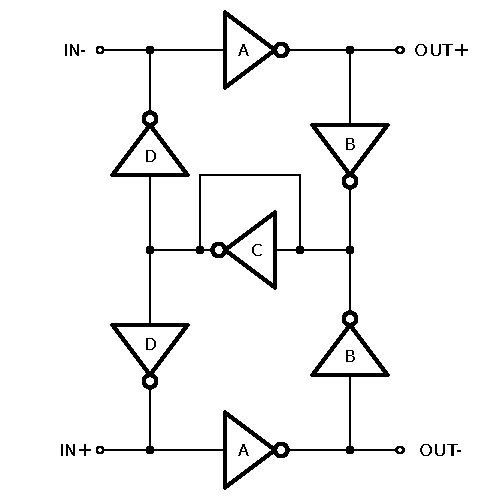
\includegraphics[scale=0.50]{circuits/vieru.pdf}}
		\caption{}
		\label{fig:vieru:sch}
	\end{subfigure}
	\caption{(a) (B)arthelemy OTA diagram\cite{barthelemy2008ota}, and (b) (V)ieru OTA circuit diagram \cite{vieru2012ultra}}
	%
\end{figure}

 The common-mode feedback technique can be used in a standalone single-stage amplifier \cite{manfredini2020ultra} by adding another node, so the output common-mode signal is fed back to the output nodes without going through the input nodes, as shown in Figure \ref{fig:manf:sch}.
 
\begin{figure}[!htbp]
	\centerline{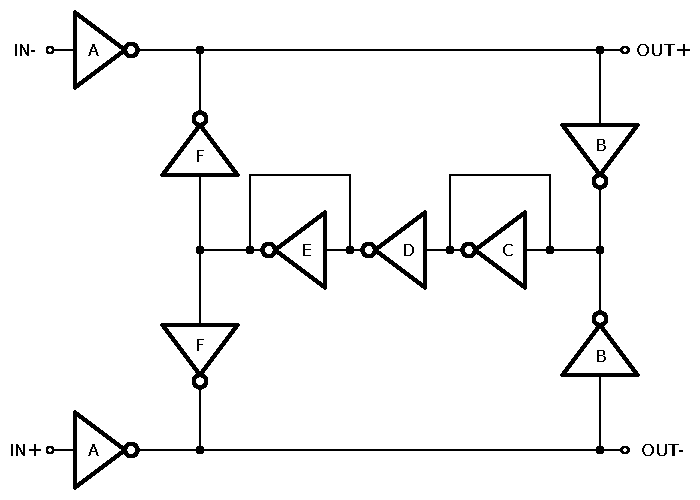
\includegraphics[scale=0.50]{circuits/manf.pdf}}
	\caption{(M)afredini OTA circuit diagram \cite{manfredini2020ultra}}
	\label{fig:manf:sch}
	%
\end{figure}


\section{Hybrid Inverter-Based Amplifier Topologies}\label{sc:hybrid}

The previously presented topologies can be merged to create hybrid designs. Figure \ref{fig:barthnauta:sch} combines the common-mode feedforward and attenuated positive feedback techniques from Barthelemy and Nauta OTAs, respectively.

\begin{figure}[!htbp]
	\centerline{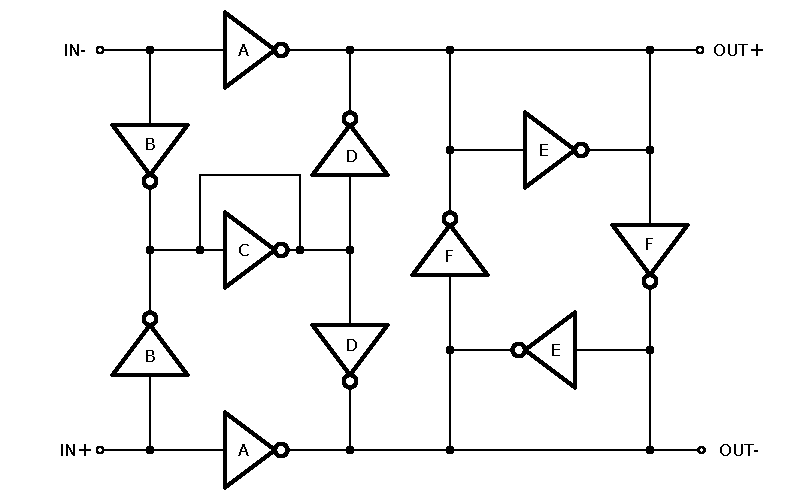
\includegraphics[scale=0.50]{circuits/barthnauta.pdf}}
	\caption{(B)arthelemy/(N)auta hybrid OTA circuit diagram}
	\label{fig:barthnauta:sch}
	%
\end{figure}

Figure \ref{fig:barthmanf:sch} shows the second hybrid topology, which uses both common-mode input feedforward and output feedback techniques, by sharing the common-mode signal path to save area and power.


%\subsection{Common-Mode Input Feedforward and Output Feedback}

\begin{figure}[!htbp]
	\centerline{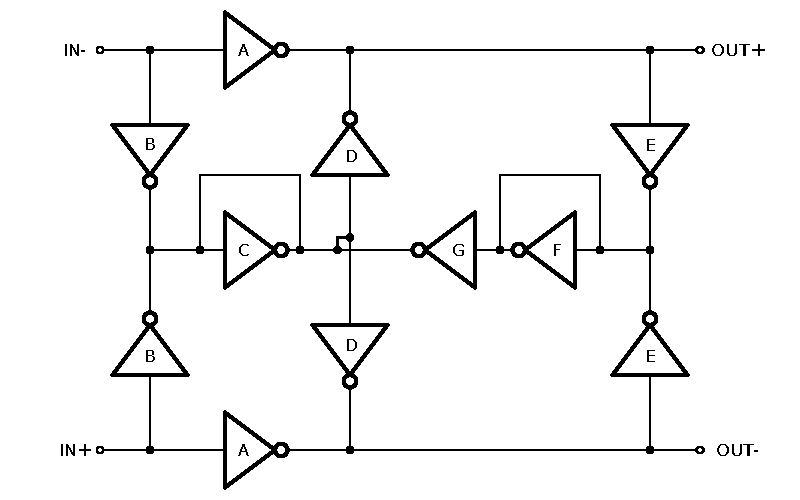
\includegraphics[scale=0.50]{circuits/barthmanf.pdf}}
	\caption{(B)arthelemy/(M)anfredini hybrid OTA circuit diagram}
	\label{fig:barthmanf:sch}
	%
\end{figure}

Figure \ref{fig:nautanauta:sch} shows a two-stage amplifier composed of two distinct Nauta stages with different multipliers and an addition Gm-C feedforward compensation path \cite{you1997multistage}.

\begin{figure}[!htbp]
	\centerline{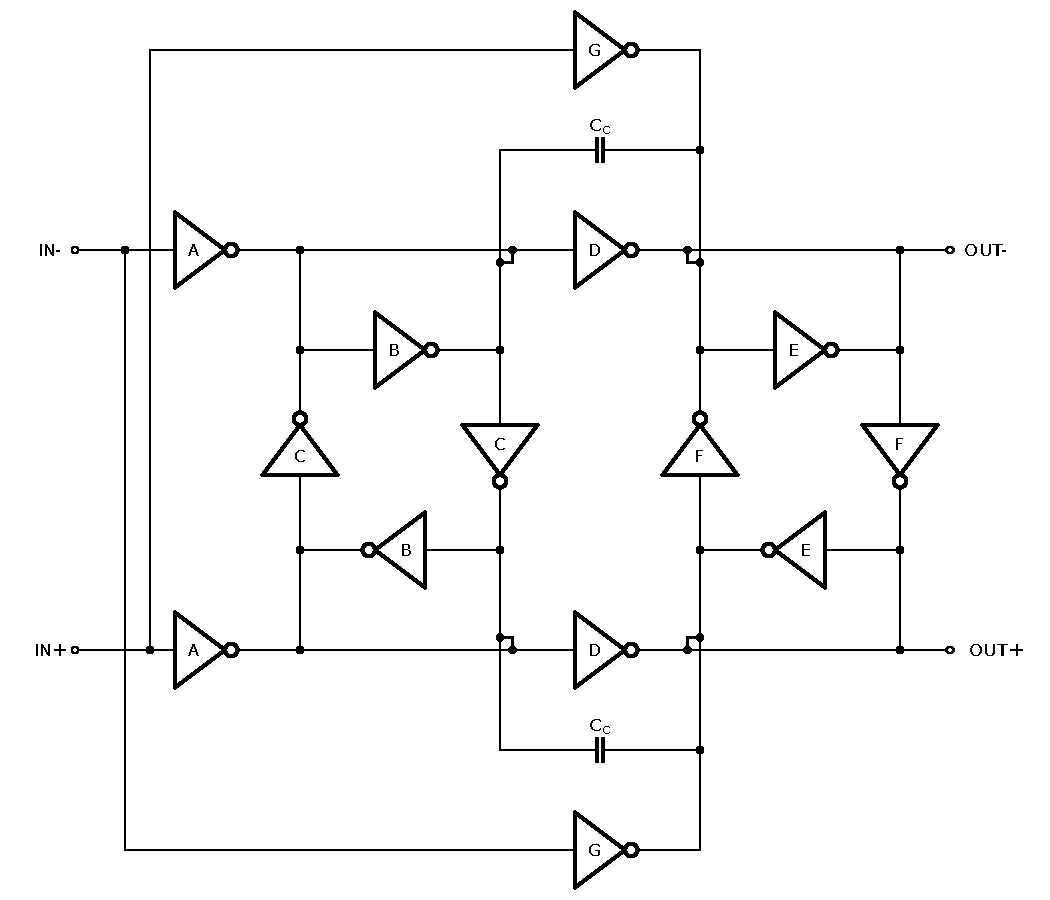
\includegraphics[scale=0.50]{circuits/nautanauta.pdf}}
	\caption{Two-stage (N)auta/(N)auta OTA circuit diagram}
	\label{fig:nautanauta:sch}
	%
\end{figure}

The second stage can be replaced by the Vieru OTA, which implements output common-mode feedback to the inner nodes, as shown in Figure \ref{fig:nautavieru:sch}.

\begin{figure}[!htbp]
	\centerline{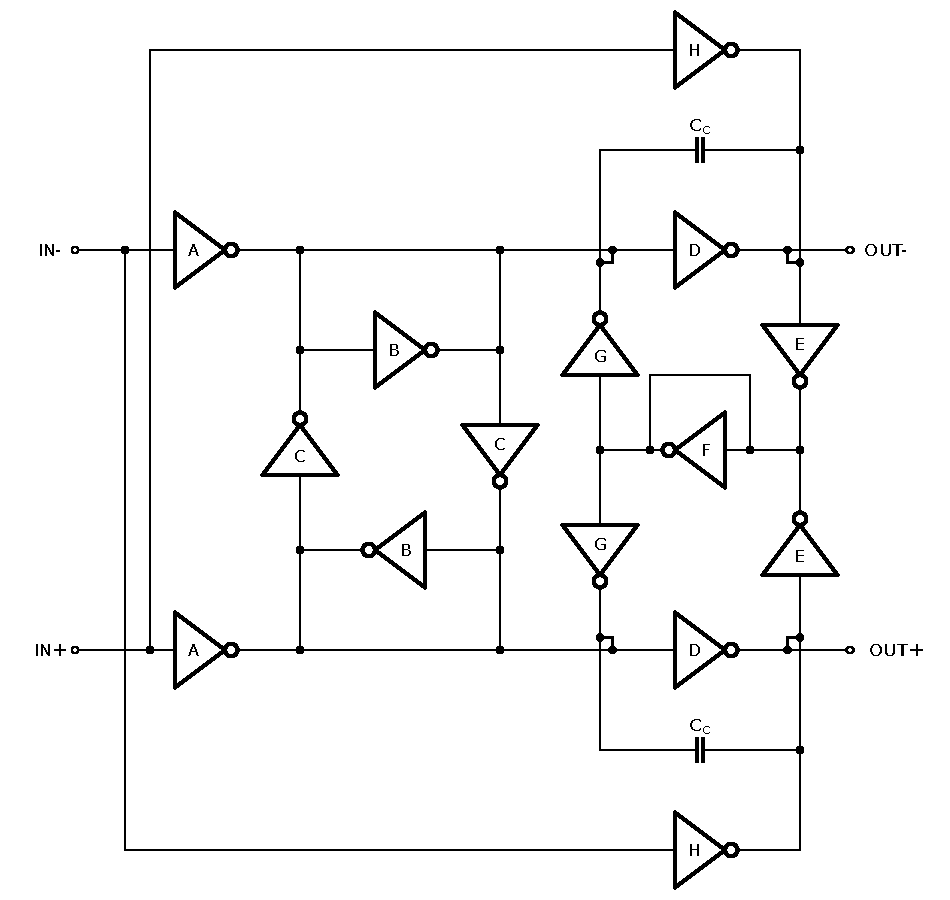
\includegraphics[scale=0.50]{circuits/nautavieru.pdf}}
	\caption{(N)auta/(V)ieru hybrid OTA circuit diagram}
	\label{fig:nautavieru:sch}
	%
\end{figure}

Another possibility is to further replace the first stage with a Manfredini stage, implement self-output common-mode feedback, and share the same path, as shown in Figure \ref{fig:manfvieru:sch}.

\begin{figure}[!htbp]
	\centerline{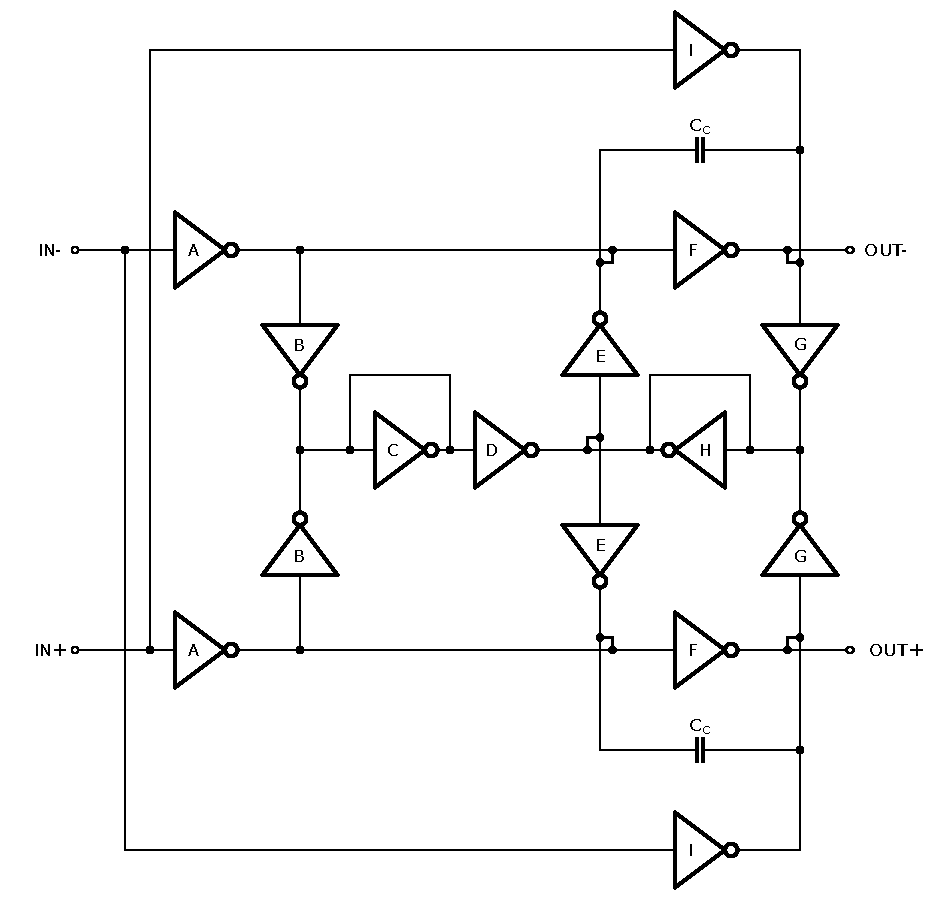
\includegraphics[scale=0.50]{circuits/manfvieru.pdf}}
	\caption{(M)anfredini/(V)ieru hybrid OTA circuit diagram}	\label{fig:manfvieru:sch}
	%
\end{figure}

%\newpage
\section{Simulation Results}\label{sc:results}

All the previous OTAs were designed and simulated using Skywater 130~nm open source PDK and open source tools. All inverters cells are identical, and they are made of two parallel P and N-type thick oxide devices with 3.0 and 1.0~μm widths, respectively, and 0.5~μm length. Each OTA individual inverter number of parallel cells is defined as in Table \ref{table:ota:sizing}.

\begin{table}[htbp]
	\caption{OTA inverter cell multipliers}\label{table:ota:sizing}
	\centering
	\begin{tabular}{l|c c c c c c c c c}
	& A & B & C & D & E & F & G & H & I \\
\hline
N   & 4 & 2 & 2 &   &   &   &   &   &   \\
B   & 4 & 2 & 4 & 4 &   &   &   &   &   \\
M   & 4 & 2 & 4 & 2 & 2 & 4 &   &   &   \\
B/N & 4 & 2 & 4 & 4 & 2 & 2 &   &   &   \\
B/V & 4 & 2 & 4 & 4 & 2 & 4 & 4 &   &   \\
N/N & 4 & 2 & 2 & 8 & 4 & 4 & 8 &   &   \\
N/V & 4 & 2 & 2 & 8 & 2 & 4 & 4 & 8 &   \\
M/V & 4 & 2 & 4 & 4 & 8 & 2 & 4 & 4 & 8 \\
		\end{tabular}
\end{table}

The simulations used as parameters typical process corner, and 3.0~V supply voltage, room temperature, and a 10~pF capacitive load ($C_L$). Table \ref{table:ota:summary} summarizes the simulation results. As all single-stage OTAs have identical A inverters, they have almost identical differential AC output voltage gain ($A_{VDF}$), gain-bandwidth-product (GBW), and phase, except for the (B)/(N) OTA, which has a slightly smaller low-frequency voltage gain, as shown in Figure \ref{fig:sim:ac}. The main difference is the common-mode voltage gain ($A_{VCM}$), as the (B) OTA has a shorter CMR bandwidth and both single-stage hybrid OTAs (B)/(N) and (B)/(M) have much lower CM voltage gain.

The DC simulation results, depicted in Figure \ref{fig:sim:dc}, shows the biggest difference between the basic (N). and the (B) and (M) OTAs, as (N) has a lower output voltage swing. Consequently, all hybrid OTAs which use the (N) technique suffers the same penalty. Finally, and obviously, the two-stage OTAs have a much larger differential voltage gain and lower phase margin (PM). The feedforward frequency compensation technique also decreases common-mode voltage gain as a side-effect. Additionally, as the designs get more complex and use more total transistors, not only their area, but their total current consumption ($I_{DD}$) increases, so their power-efficiency Figure of Merit (FoM) decreases as well.

\begin{table}[htbp]
	\caption{OTA inverter cell multipliers}\label{table:ota:summary}
	\centering
	\begin{tabular}{l|r r r r r r }
		& $A_{VDF}$ & $A_{VCM}$ & GBW   & $I_{DD}$ & P.M. & FoM      \\
		& (dB)      & (dB)      & (MHz) & (mA)     & (°)  & V$^{-1}$ \\
		\hline
		N   & 19.6 &  -0.9 &  33.4 & 1.74 & 96 & 19.3 \\
		B   & 19.6 &  -0.9 &  33.5 & 2.60 & 96 & 12.9 \\
		M   & 19.6 &   0.7 &  33.5 & 3.04 & 96 & 11.0 \\
		B/N & 16.1 & -21.8 &  33.1 & 3.47 & 99 &  9.5 \\
		B/V & 19.6 & -16.3 &  33.5 & 3.91 & 96 &  8.6 \\
		N/N & 36.6 & -21.8 &  92.2 & 6.94 & 60 & 13.3 \\
		N/V & 37.0 & -16.3 &  92.9 & 6.94 & 62 & 13.4 \\
		M/V & 40.1 & -18.6 &  94.9 & 7.38 & 59 & 12.7 \\
	\end{tabular}
	\footnotesize{\\FoM = $100\times$GBW$\times C_L / I_{DD}$}
\end{table}

\begin{figure*}[!htbp]
	\tikzsetnextfilename{ac}
\begin{tikzpicture}

\begin{scope}[shift={(0.0cm,-0.0cm)}]
\begin{semilogxaxis}[
%	xlabel={Frequency [Hz]},
	ylabel={Differential gain (dB)},
	xmin=1e3, xmax=1e12,
	ymin=-70, ymax=50,
	xtick={1e3,1e6,1e9,1e12},
	ytick={-60,-40,-20,0,20,40},
	%        yticklabel style={/pgf/number format/.cd,fixed,fixed zerofill,precision=0},
	legend pos=south west,
	legend columns=1,
	width  = 6.5cm,
	height = 4.0cm    
	]
	
	\addplot [
	color=red,
	no marks,
	mark repeat = 6,
	mark phase = 1,
	solid
	]
	table [each nth point={1}, x expr=\thisrowno{0}, y expr=\thisrowno{1}, col sep=comma]
	{./data/ac_df_av.csv};
	\addlegendentry{N}
	
	\addplot [
	color=blue,
	no marks,
	mark repeat = 6,
	mark phase = 1,
	dashed
	]
	table [each nth point={1}, x expr=\thisrowno{0}, y expr=\thisrowno{3}, col sep=comma]
	{./data/ac_df_av.csv};
	\addlegendentry{B}
	
	\addplot [
	color=green,
	no marks,
	mark repeat = 6,
	mark phase = 1,
	dotted
	]
	table [each nth point={1}, x expr=\thisrowno{0}, y expr=\thisrowno{5}, col sep=comma]
	{./data/ac_df_av.csv};
	\addlegendentry{M}
	
\end{semilogxaxis}
\end{scope}

\begin{scope}[shift={(0.0cm,-3.0cm)}]	
	\begin{semilogxaxis}[
%		xlabel={Frequency [Hz]},
		ylabel={Phase (°)},
		xmin=1e3, xmax=1e12,
		ymin=-45, ymax=225,
		xtick={1e3,1e6,1e9,1e12},
		ytick={180,90,0},
		%        yticklabel style={/pgf/number format/.cd,fixed,fixed zerofill,precision=0},
		legend pos=south west,
		legend columns=1,
		width  = 6.5cm,
		height = 4.0cm    
		]
		
		\addplot [
		color=red,
		no marks,
		mark repeat = 6,
		mark phase = 1,
		solid
		]
		table [each nth point={1}, x expr=\thisrowno{0}, y expr=\thisrowno{1}, col sep=comma]
		{./data/ac_df_ph.csv};
		\addlegendentry{N}
		
		\addplot [
		color=blue,
		no marks,
		mark repeat = 6,
		mark phase = 1,
		dashed
		]
		table [each nth point={1}, x expr=\thisrowno{0}, y expr=\thisrowno{3}, col sep=comma]
		{./data/ac_df_ph.csv};
		\addlegendentry{B}
		
		\addplot [
		color=green,
		no marks,
		mark repeat = 6,
		mark phase = 1,
		dotted
		]
		table [each nth point={1}, x expr=\thisrowno{0}, y expr=\thisrowno{5}, col sep=comma]
		{./data/ac_df_ph.csv};
	\addlegendentry{M}
		
\end{semilogxaxis}
\end{scope}

\begin{scope}[shift={(0.0cm,-6.0cm)}]	
\begin{semilogxaxis}[
    xlabel={Frequency (Hz)},
    ylabel={Common-mode gain (dB)},
    xmin=1e3, xmax=1e12,
	ymin=-70, ymax=50,
	xtick={1e3,1e6,1e9,1e12},
	ytick={-60,-40,-20,0,20,40},
%        yticklabel style={/pgf/number format/.cd,fixed,fixed zerofill,precision=0},
    legend pos=north east,
    legend columns=1,
    width  = 6.5cm,
    height = 4.0cm    
]

\addplot [
    color=red,
    no marks,
    mark repeat = 6,
    mark phase = 1,
    solid
    ]
    table [each nth point={1}, x expr=\thisrowno{0}, y expr=\thisrowno{1}, col sep=comma]
	{./data/ac_cm_av.csv};
\addlegendentry{N}

\addplot [
	color=blue,
	no marks,
	mark repeat = 6,
	mark phase = 1,
	dashed
]
	table [each nth point={1}, x expr=\thisrowno{0}, y expr=\thisrowno{3}, col sep=comma]
	{./data/ac_cm_av.csv};
\addlegendentry{B}

\addplot [
	color=green,
	no marks,
	mark repeat = 6,
	mark phase = 1,
	dotted
	]
	table [each nth point={1}, x expr=\thisrowno{0}, y expr=\thisrowno{5}, col sep=comma]
	{./data/ac_cm_av.csv};
\addlegendentry{M}

\end{semilogxaxis}
\end{scope}

\begin{scope}[shift={(6.0cm,-0.0cm)}]
	\begin{semilogxaxis}[
		%	xlabel={Frequency [Hz]},
%		ylabel={Differential gain [dB]},
		xmin=1e3, xmax=1e12,
		ymin=-70, ymax=50,
		xtick={1e3,1e6,1e9,1e12},
		ytick={-60,-40,-20,0,20,40},
		%        yticklabel style={/pgf/number format/.cd,fixed,fixed zerofill,precision=0},
		legend pos=south west,
		legend columns=1,
		width  = 6.5cm,
		height = 4.0cm    
		]
		
		\addplot [
		color=red,
		no marks,
		mark repeat = 6,
		mark phase = 1,
		solid
		]
		table [each nth point={1}, x expr=\thisrowno{0}, y expr=\thisrowno{1}, col sep=comma]
		{./data/ac_df_av.csv};
		\addlegendentry{N}
		
		\addplot [
		color=blue,
		no marks,
		mark repeat = 6,
		mark phase = 1,
		dashed
		]
		table [each nth point={1}, x expr=\thisrowno{0}, y expr=\thisrowno{7}, col sep=comma]
		{./data/ac_df_av.csv};
		\addlegendentry{B/N}
		
		\addplot [
		color=green,
		no marks,
		mark repeat = 6,
		mark phase = 1,
		dotted
		]
		table [each nth point={1}, x expr=\thisrowno{0}, y expr=\thisrowno{9}, col sep=comma]
		{./data/ac_df_av.csv};
		\addlegendentry{B/M}
		
	\end{semilogxaxis}
\end{scope}

\begin{scope}[shift={(6.0cm,-3.0cm)}]	
	\begin{semilogxaxis}[
		%		xlabel={Frequency [Hz]},
%		ylabel={Phase [°]},
		xmin=1e3, xmax=1e12,
		ymin=-45, ymax=225,
		xtick={1e3,1e6,1e9,1e12},
		ytick={180,90,0},
		%        yticklabel style={/pgf/number format/.cd,fixed,fixed zerofill,precision=0},
		legend pos=south west,
		legend columns=1,
		width  = 6.5cm,
		height = 4.0cm    
		]
		
		\addplot [
		color=red,
		no marks,
		mark repeat = 6,
		mark phase = 1,
		solid
		]
		table [each nth point={1}, x expr=\thisrowno{0}, y expr=\thisrowno{1}, col sep=comma]
		{./data/ac_df_ph.csv};
		\addlegendentry{N}
		
		\addplot [
		color=blue,
		no marks,
		mark repeat = 6,
		mark phase = 1,
		dashed
		]
		table [each nth point={1}, x expr=\thisrowno{0}, y expr=\thisrowno{7}, col sep=comma]
		{./data/ac_df_ph.csv};
		\addlegendentry{B/N}
		
		\addplot [
		color=green,
		no marks,
		mark repeat = 6,
		mark phase = 1,
		dotted
		]
		table [each nth point={1}, x expr=\thisrowno{0}, y expr=\thisrowno{9}, col sep=comma]
		{./data/ac_df_ph.csv};
		\addlegendentry{B/M}
		
	\end{semilogxaxis}
\end{scope}

\begin{scope}[shift={(6.0cm,-6.0cm)}]	
	\begin{semilogxaxis}[
		xlabel={Frequency (Hz)},
%		ylabel={Common-mode gain [dB]},
		xmin=1e3, xmax=1e12,
		ymin=-70, ymax=50,
		xtick={1e3,1e6,1e9,1e12},
		ytick={-60,-40,-20,0,20,40},
		%        yticklabel style={/pgf/number format/.cd,fixed,fixed zerofill,precision=0},
		legend pos=north east,
		legend columns=1,
		width  = 6.5cm,
		height = 4.0cm    
		]
		
		\addplot [
		color=red,
		no marks,
		mark repeat = 6,
		mark phase = 1,
		solid
		]
		table [each nth point={1}, x expr=\thisrowno{0}, y expr=\thisrowno{1}, col sep=comma]
		{./data/ac_cm_av.csv};
		\addlegendentry{N}
		
		\addplot [
		color=blue,
		no marks,
		mark repeat = 6,
		mark phase = 1,
		dashed
		]
		table [each nth point={1}, x expr=\thisrowno{0}, y expr=\thisrowno{7}, col sep=comma]
		{./data/ac_cm_av.csv};
		\addlegendentry{B/N}
		
		\addplot [
		color=green,
		no marks,
		mark repeat = 6,
		mark phase = 1,
		dotted
		]
		table [each nth point={1}, x expr=\thisrowno{0}, y expr=\thisrowno{9}, col sep=comma]
		{./data/ac_cm_av.csv};
		\addlegendentry{B/M}
		
	\end{semilogxaxis}
\end{scope}

\begin{scope}[shift={(12.0cm,-0.0cm)}]
	\begin{semilogxaxis}[
%	xlabel={Frequency [Hz]},
%		ylabel={Differential gain [dB]},
		xmin=1e3, xmax=1e12,
		ymin=-70, ymax=50,
		xtick={1e3,1e6,1e9,1e12},
		ytick={-60,-40,-20,0,20,40},
		%        yticklabel style={/pgf/number format/.cd,fixed,fixed zerofill,precision=0},
		legend pos=south west,
		legend columns=1,
		width  = 6.5cm,
		height = 4.0cm    
		]
		
		\addplot [
		color=red,
		no marks,
		mark repeat = 6,
		mark phase = 1,
		solid
		]
		table [each nth point={1}, x expr=\thisrowno{0}, y expr=\thisrowno{11}, col sep=comma]
		{./data/ac_df_av.csv};
		\addlegendentry{N/N}
		
		\addplot [
		color=blue,
		no marks,
		mark repeat = 6,
		mark phase = 1,
		dashed
		]
		table [each nth point={1}, x expr=\thisrowno{0}, y expr=\thisrowno{13}, col sep=comma]
		{./data/ac_df_av.csv};
		\addlegendentry{N/V}
		
		\addplot [
		color=green,
		no marks,
		mark repeat = 6,
		mark phase = 1,
		dotted
		]
		table [each nth point={1}, x expr=\thisrowno{0}, y expr=\thisrowno{15}, col sep=comma]
		{./data/ac_df_av.csv};
		\addlegendentry{M/V}
		
	\end{semilogxaxis}
\end{scope}

\begin{scope}[shift={(12.0cm,-3.0cm)}]	
	\begin{semilogxaxis}[
%		xlabel={Frequency [Hz]},
%		ylabel={Phase [°]},
		xmin=1e3, xmax=1e12,
		ymin=-45, ymax=225,
		xtick={1e3,1e6,1e9,1e12},
		ytick={180,90,0},
		%        yticklabel style={/pgf/number format/.cd,fixed,fixed zerofill,precision=0},
		legend pos=south west,
		legend columns=1,
		width  = 6.5cm,
		height = 4.0cm    
		]
		
		\addplot [
		color=red,
		no marks,
		mark repeat = 6,
		mark phase = 1,
		solid
		]
		table [each nth point={1}, x expr=\thisrowno{0}, y expr=\thisrowno{11}, col sep=comma]
		{./data/ac_df_ph.csv};
		\addlegendentry{N/N}
		
		\addplot [
		color=blue,
		no marks,
		mark repeat = 6,
		mark phase = 1,
		dashed
		]
		table [each nth point={1}, x expr=\thisrowno{0}, y expr=\thisrowno{13}, col sep=comma]
		{./data/ac_df_ph.csv};
		\addlegendentry{N/V}
		
		\addplot [
		color=green,
		no marks,
		mark repeat = 6,
		mark phase = 1,
		dotted
		]
		table [each nth point={1}, x expr=\thisrowno{0}, y expr=\thisrowno{15}, col sep=comma]
		{./data/ac_df_ph.csv};
		\addlegendentry{M/V}
		
	\end{semilogxaxis}
\end{scope}

\begin{scope}[shift={(12.0cm,-6.0cm)}]	
	\begin{semilogxaxis}[
		xlabel={Frequency (Hz)},
%		ylabel={Common-mode gain [dB]},
		xmin=1e3, xmax=1e12,
		ymin=-70, ymax=50,
		xtick={1e3,1e6,1e9,1e12},
		ytick={-60,-40,-20,0,20,40},
		%        yticklabel style={/pgf/number format/.cd,fixed,fixed zerofill,precision=0},
		legend pos=north east,
		legend columns=2,
		width  = 6.5cm,
		height = 4.0cm    
		]
		
		\addplot [
		color=red,
		no marks,
		mark repeat = 6,
		mark phase = 1,
		solid
		]
		table [each nth point={1}, x expr=\thisrowno{0}, y expr=\thisrowno{11}, col sep=comma]
		{./data/ac_cm_av.csv};
		\addlegendentry{N/N}
		
		\addplot [
		color=blue,
		no marks,
		mark repeat = 6,
		mark phase = 1,
		dashed
		]
		table [each nth point={1}, x expr=\thisrowno{0}, y expr=\thisrowno{13}, col sep=comma]
		{./data/ac_cm_av.csv};
		\addlegendentry{N/V}
		
		\addplot [
		color=green,
		no marks,
		mark repeat = 6,
		mark phase = 1,
		dotted
		]
		table [each nth point={1}, x expr=\thisrowno{0}, y expr=\thisrowno{15}, col sep=comma]
		{./data/ac_cm_av.csv};
		\addlegendentry{M/V}
		
	\end{semilogxaxis}
\end{scope}

\end{tikzpicture}

	\caption{AC simulation results}
	\label{fig:sim:ac}
	%
\end{figure*}

\begin{figure*}[!htbp]
	\tikzsetnextfilename{dc}
\begin{tikzpicture}

\begin{scope}[shift={(0.0cm,-0.0cm)}]
\begin{axis}[
	xlabel={Diff. input voltage (V)},
	ylabel={Diff. output voltage (V)},
	xmin=-0.4, xmax=0.4,
	ymin=-3, ymax=3,
%	xtick={-1,-0.5,0,0.5,1},
	xtick={-0.4,-0.2,0,0.2,0.4},
	ytick={-3,-1.5,0,1.5,3},
	yticklabel style={/pgf/number format/.cd,fixed,fixed zerofill,precision=1},
	legend pos=north west,
	legend columns=1,
	width  = 6.5cm,
	height = 4.0cm    
	]
	
	\addplot [
	color=red,
	no marks,
	mark repeat = 6,
	mark phase = 1,
	solid
	]
	table [each nth point={1}, x expr=\thisrowno{1}, y expr=\thisrowno{3}, col sep=comma]
	{./data/dc_df_vo.csv};
	\addlegendentry{N}
	
	\addplot [
	color=blue,
	no marks,
	mark repeat = 6,
	mark phase = 1,
	dashed
	]
	table [each nth point={1}, x expr=\thisrowno{1}, y expr=\thisrowno{5}, col sep=comma]
	{./data/dc_df_vo.csv};
	\addlegendentry{B}
	
	\addplot [
	color=green,
	no marks,
	mark repeat = 6,
	mark phase = 1,
	dotted
	]
	table [each nth point={1}, x expr=\thisrowno{1}, y expr=\thisrowno{7}, col sep=comma]
	{./data/dc_df_vo.csv};
	\addlegendentry{M}
	
\end{axis}
\end{scope}

\begin{scope}[shift={(0.0cm,-3.5cm)}]	
	\begin{axis}[
		xlabel={Diff. output voltage (V)},
		ylabel={Diff. gain (dB)},
		xmin=-3, xmax=3,
		ymin=-50, ymax=50,
		xtick={-3,-1.5,0,1.5,3},
		ytick={-40,-20,0,20,40},
		%        yticklabel style={/pgf/number format/.cd,fixed,fixed zerofill,precision=0},
		legend pos=south west,
		legend columns=3,
		width  = 6.5cm,
		height = 4.0cm    
		]
		
		\addplot [
		color=red,
		no marks,
		mark repeat = 6,
		mark phase = 1,
		solid
		]
		table [each nth point={1}, x expr=\thisrowno{1}, y expr={20*log10(\thisrowno{3})}, col sep=comma]
		{./data/dc_df_av.csv};
		\addlegendentry{N}
		
		\addplot [
		color=blue,
		no marks,
		mark repeat = 6,
		mark phase = 1,
		dashed
		]
		table [each nth point={1}, x expr=\thisrowno{5}, y expr={20*log10(\thisrowno{7})}, col sep=comma]
		{./data/dc_df_av.csv};
		\addlegendentry{B}
		
		\addplot [
		color=green,
		no marks,
		mark repeat = 6,
		mark phase = 1,
		dotted
		]
		table [each nth point={1}, x expr=\thisrowno{9}, y expr={20*log10(\thisrowno{11})}, col sep=comma]
		{./data/dc_df_av.csv};
	\addlegendentry{M}
		
\end{axis}
\end{scope}

\begin{scope}[shift={(0.0cm,-7.0cm)}]
	\begin{axis}[
		xlabel={CM input voltage (V)},
		ylabel={CM output voltage (V)},
		xmin=0, xmax=3,
		ymin=0, ymax=3,
		xtick={0,-0.5,1,1.5,2,2.5,3},
		xtick={0,-0.5,1,1.5,2,2.5,3},
		yticklabel style={/pgf/number format/.cd,fixed,fixed zerofill,precision=1},
		legend pos=south west,
		legend columns=3,
		width  = 6.5cm,
		height = 4.0cm    
		]
		
		\addplot [
		color=red,
		no marks,
		mark repeat = 6,
		mark phase = 1,
		solid
		]
		table [each nth point={1}, x expr=\thisrowno{0}, y expr=\thisrowno{1}, col sep=comma]
		{./data/dc_cm_vo.csv};
		\addlegendentry{N}
		
		\addplot [
		color=blue,
		no marks,
		mark repeat = 6,
		mark phase = 1,
		dashed
		]
		table [each nth point={1}, x expr=\thisrowno{0}, y expr=\thisrowno{3}, col sep=comma]
		{./data/dc_cm_vo.csv};
		\addlegendentry{B}
		
		\addplot [
		color=green,
		no marks,
		mark repeat = 6,
		mark phase = 1,
		dotted
		]
		table [each nth point={1}, x expr=\thisrowno{0}, y expr=\thisrowno{5}, col sep=comma]
		{./data/dc_cm_vo.csv};
		\addlegendentry{M}
		
	\end{axis}
\end{scope}

\begin{scope}[shift={(6.0cm,-0.0cm)}]
	\begin{axis}[
		xlabel={Diff input voltage (V)},
%		ylabel={Output voltage (dB)},
		xmin=-0.4, xmax=0.4,
		ymin=-3, ymax=3,
%		xtick={-1,-0.5,0,0.5,1},
		xtick={-0.4,-0.2,0,0.2,0.4},		
		ytick={-3,-1.5,0,1.5,3},
		yticklabel style={/pgf/number format/.cd,fixed,fixed zerofill,precision=1},
		legend pos=north west,
		legend columns=1,
		width  = 6.5cm,
		height = 4.0cm    
		]
		
		\addplot [
		color=red,
		no marks,
		mark repeat = 6,
		mark phase = 1,
		solid
		]
		table [each nth point={1}, x expr=\thisrowno{1}, y expr=\thisrowno{3}, col sep=comma]
		{./data/dc_df_vo.csv};
		\addlegendentry{N}
		
		\addplot [
		color=blue,
		no marks,
		mark repeat = 6,
		mark phase = 1,
		dashed
		]
		table [each nth point={1}, x expr=\thisrowno{1}, y expr=\thisrowno{9}, col sep=comma]
		{./data/dc_df_vo.csv};
		\addlegendentry{B/N}
		
		\addplot [
		color=green,
		no marks,
		mark repeat = 6,
		mark phase = 1,
		dotted
		]
		table [each nth point={1}, x expr=\thisrowno{1}, y expr=\thisrowno{11}, col sep=comma]
		{./data/dc_df_vo.csv};
		\addlegendentry{B/M}
		
	\end{axis}
\end{scope}

\begin{scope}[shift={(6.0cm,-3.5cm)}]	
	\begin{axis}[
		xlabel={Diff. output voltage (V)},
%		ylabel={Differential Gain (dB)},
		xmin=-3, xmax=3,
		ymin=-50, ymax=50,
		xtick={-3,-1.5,0,1.5,3},
		ytick={-40,-20,0,20,40},
		%        yticklabel style={/pgf/number format/.cd,fixed,fixed zerofill,precision=0},
		legend pos=south west,
		legend columns=3,
		width  = 6.5cm,
		height = 4.0cm    
		]
		
		\addplot [
		color=red,
		no marks,
		mark repeat = 6,
		mark phase = 1,
		solid
		]
		table [each nth point={1}, x expr=\thisrowno{1}, y expr={20*log10(\thisrowno{3})}, col sep=comma]
		{./data/dc_df_av.csv};
		\addlegendentry{N}
		
		\addplot [
		color=blue,
		no marks,
		mark repeat = 6,
		mark phase = 1,
		dashed
		]
		table [each nth point={1}, x expr=\thisrowno{13}, y expr={20*log10(\thisrowno{15})}, col sep=comma]
		{./data/dc_df_av.csv};
		\addlegendentry{B/N}
		
		\addplot [
		color=green,
		no marks,
		mark repeat = 6,
		mark phase = 1,
		dotted
		]
		table [each nth point={1}, x expr=\thisrowno{17}, y expr={20*log10(\thisrowno{19})}, col sep=comma]
		{./data/dc_df_av.csv};
		\addlegendentry{B/M}
		
	\end{axis}
\end{scope}

\begin{scope}[shift={(6.0cm,-7.0cm)}]
	\begin{axis}[
		xlabel={CM input voltage (V)},
%		ylabel={Output voltage (V)},
		xmin=0, xmax=3,
		ymin=0, ymax=3,
		xtick={0,0.5,1,1.5,2,2.5,3},
		ytick={0,0.5,1,1.5,2,2.5,3},
		yticklabel style={/pgf/number format/.cd,fixed,fixed zerofill,precision=1},
		legend pos=south west,
		legend columns=3,
		width  = 6.5cm,
		height = 4.0cm    
		]
		
		\addplot [
		color=red,
		no marks,
		mark repeat = 6,
		mark phase = 1,
		solid
		]
		table [each nth point={1}, x expr=\thisrowno{0}, y expr=\thisrowno{1}, col sep=comma]
		{./data/dc_cm_vo.csv};
		\addlegendentry{N}
		
		\addplot [
		color=blue,
		no marks,
		mark repeat = 6,
		mark phase = 1,
		dashed
		]
		table [each nth point={1}, x expr=\thisrowno{0}, y expr=\thisrowno{7}, col sep=comma]
		{./data/dc_cm_vo.csv};
		\addlegendentry{B/N}
		
		\addplot [
		color=green,
		no marks,
		mark repeat = 6,
		mark phase = 1,
		dotted
		]
		table [each nth point={1}, x expr=\thisrowno{0}, y expr=\thisrowno{9}, col sep=comma]
		{./data/dc_cm_vo.csv};
		\addlegendentry{B/M}
		
	\end{axis}
\end{scope}

\begin{scope}[shift={(12.0cm,-0.0cm)}]
	\begin{axis}[
		xlabel={Diff. input voltage (V)},
		%		ylabel={Output voltage (dB)},
		xmin=-0.4, xmax=0.4,
		ymin=-3, ymax=3,
%		xtick={-1,-0.5,0,0.5,1},
		xtick={-0.4,-0.2,0,0.2,0.4},
		ytick={-3,-1.5,0,1.5,3},
		yticklabel style={/pgf/number format/.cd,fixed,fixed zerofill,precision=1},
		legend pos=north west,
		legend columns=1,
		width  = 6.5cm,
		height = 4.0cm    
		]
		
		\addplot [
		color=red,
		no marks,
		mark repeat = 6,
		mark phase = 1,
		solid
		]
		table [each nth point={1}, x expr=\thisrowno{1}, y expr=\thisrowno{13}, col sep=comma]
		{./data/dc_df_vo.csv};
		\addlegendentry{N/N}
		
		\addplot [
		color=blue,
		no marks,
		mark repeat = 6,
		mark phase = 1,
		dashed
		]
		table [each nth point={1}, x expr=\thisrowno{1}, y expr=\thisrowno{15}, col sep=comma]
		{./data/dc_df_vo.csv};
		\addlegendentry{N/V}
		
		\addplot [
		color=green,
		no marks,
		mark repeat = 6,
		mark phase = 1,
		dotted
		]
		table [each nth point={1}, x expr=\thisrowno{1}, y expr=\thisrowno{17}, col sep=comma]
		{./data/dc_df_vo.csv};
		\addlegendentry{M/V}
		
	\end{axis}
\end{scope}

\begin{scope}[shift={(12.0cm,-3.5cm)}]	
	\begin{axis}[
		xlabel={Diff. output voltage (V)},
		%		ylabel={Differential Gain (dB)},
		xmin=-3, xmax=3,
		ymin=-50, ymax=50,
		xtick={-3,-1.5,0,1.5,3},
		ytick={-40,-20,0,20,40},
		%        yticklabel style={/pgf/number format/.cd,fixed,fixed zerofill,precision=0},
		legend pos=south west,
		legend columns=3,
		width  = 6.5cm,
		height = 4.0cm    
		]
		
		\addplot [
		color=red,
		no marks,
		mark repeat = 6,
		mark phase = 1,
		solid
		]
		table [each nth point={1}, x expr=\thisrowno{21}, y expr={20*log10(\thisrowno{23})}, col sep=comma]
		{./data/dc_df_av.csv};
		\addlegendentry{N/N}
		
		\addplot [
		color=blue,
		no marks,
		mark repeat = 6,
		mark phase = 1,
		dashed
		]
		table [each nth point={1}, x expr=\thisrowno{25}, y expr={20*log10(\thisrowno{27})}, col sep=comma]
		{./data/dc_df_av.csv};
		\addlegendentry{N/V}
		
		\addplot [
		color=green,
		no marks,
		mark repeat = 6,
		mark phase = 1,
		dotted
		]
		table [each nth point={1}, x expr=\thisrowno{29}, y expr={20*log10(\thisrowno{31})}, col sep=comma]
		{./data/dc_df_av.csv};
		\addlegendentry{M/V}
		
	\end{axis}
\end{scope}

\begin{scope}[shift={(12.0cm,-7.0cm)}]
	\begin{axis}[
		xlabel={CM input voltage (V)},
%		ylabel={Output voltage (V)},
		xmin=0, xmax=3,
		ymin=0, ymax=3,
		xtick={0,0.5,1,1.5,2,2.5,3},
		ytick={0,0.5,1,1.5,2,2.5,3},
		yticklabel style={/pgf/number format/.cd,fixed,fixed zerofill,precision=1},
		legend pos=south west,
		legend columns=3,
		width  = 6.5cm,
		height = 4.0cm    
		]
		
		\addplot [
		color=red,
		no marks,
		mark repeat = 6,
		mark phase = 1,
		solid
		]
		table [each nth point={1}, x expr=\thisrowno{0}, y expr=\thisrowno{11}, col sep=comma]
		{./data/dc_cm_vo.csv};
		\addlegendentry{N/N}
		
		\addplot [
		color=blue,
		no marks,
		mark repeat = 6,
		mark phase = 1,
		dashed
		]
		table [each nth point={1}, x expr=\thisrowno{0}, y expr=\thisrowno{13}, col sep=comma]
		{./data/dc_cm_vo.csv};
		\addlegendentry{N/V}
		
		\addplot [
		color=green,
		no marks,
		mark repeat = 6,
		mark phase = 1,
		dotted
		]
		table [each nth point={1}, x expr=\thisrowno{0}, y expr=\thisrowno{15}, col sep=comma]
		{./data/dc_cm_vo.csv};
		\addlegendentry{M/V}
		
	\end{axis}
\end{scope}


\end{tikzpicture}

	\caption{DC simulation results}
	\label{fig:sim:dc}
	%
\end{figure*}

%	\FloatBarrier
	\section{Conclusion}\label{section:conclusion}

The Nauta inverter-based OTA topology is, without doubt, the most power-efficient one, but its drawbacks are lower output swing. The other basic topologies, proposed by Barthelemy, Manfredini, and Vieru solve that by increasing the OTA complexity. Hybrid topologies merge those techniques and share paths, saving power and area while retaining the output swing of those alternative basic topologies. Feedforward active frequency compensation makes two-stage amplifiers stable, and as bonus, it also improves common-mode rejection.
		
	\section*{Acknowledgment}
	
The authors would like to thank Google, eFabless and Skywater Foundry for the open source PDK and tools.
	

% References

	\bibliographystyle{IEEEtran}
	\bibliography{main}
	
	
\end{document}
